\section*{Metodyka testów}
Efekty treningu sieci zostaną przetestowane na 3 zbiorach danych:
\begin{itemize}
    \item zbiór testowy MNIST (10000 elementów) - oznaczony $ZT1$
    \item zbiór testowy stworzony przeze mnie (30 elementów) - oznaczony $ZT2$
    \item zbiór testowy stworzony przez osobę trzecią (30 elementów) - oznaczony $ZT3$
\end{itemize}
Zbiór MNIST został przygotowany w postaci odpowiedniej dla sieci neuronowej, natomiast zbiory $ZT2$ i $ZT3$ muszą zostać odpowiednio zmienione. W wersji podstawowej, dla każdego obrazu został zwiększony kontrast, następnie zmieniono RGB na skalę szarości, oraz zmapowano wartości pixeli na $0$ lub $1$. Finalnie obrazy zostały zeskalowane do rozmiaru 28 x 28. Dodatkowo, dla każdego ze zbiorów $ZT2$ i $ZT3$ został stworzony dodatkowy zbiór (odpowiednio $ZT2\_PREPROCESSED$ i $ZT3\_PREPROCESSED$), który dokładniej przystosował zdjęcia na potrzeby sieci. Z każdego zdjęcia została wycięta część zawierająca cyfrę, następne zeskalowana do 20px, oraz wstawiona w obraz 28 x 28.

\begin{figure}[!htb]
\minipage{0.32\textwidth}
    \centering
    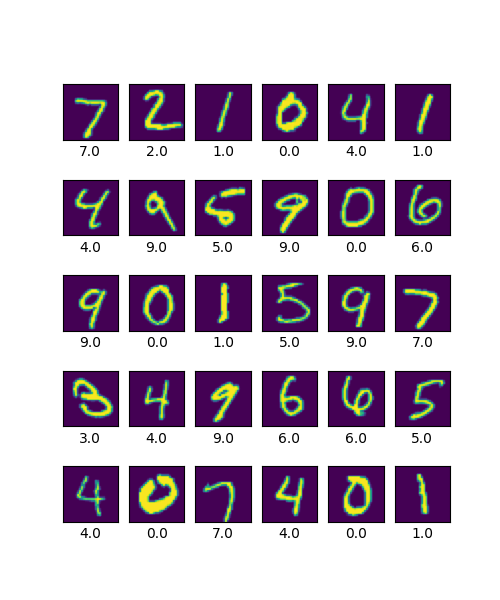
\includegraphics[width=\linewidth]{dataset_mnist.png}
    $ZT1$
\endminipage\hfill
\minipage{0.32\textwidth}
    \centering
    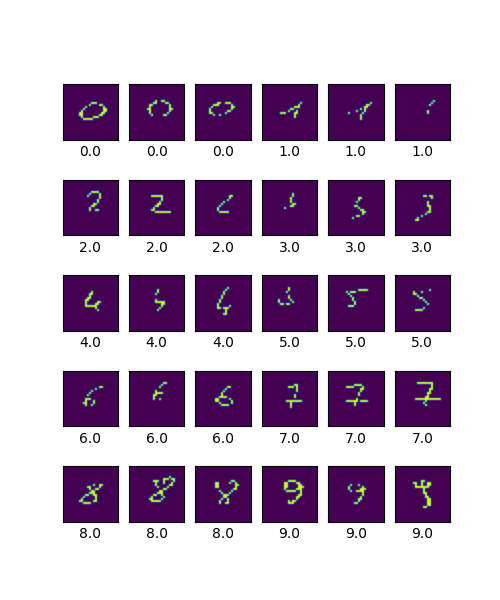
\includegraphics[width=\linewidth]{dataset_my.png}
    $ZT2$
\endminipage\hfill
\minipage{0.32\textwidth}
    \centering
    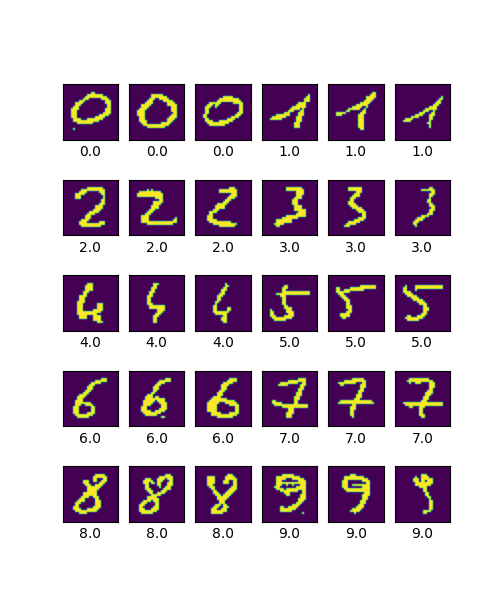
\includegraphics[width=\linewidth]{dataset_my_preprocessed.png}
    $ZT2\_PREPROCESSED$
\endminipage
\end{figure}

\section*{Wybór parametrów}
Początkowe parametry do wyboru struktury sieci to:
\begin{itemize}
    \item batch\_size = 8
    \item epochs = 10
    \item optimizer = adam
    \item loss = Sparse Categorical Crossentropy
\end{itemize}
Każda sieć przyjmuje input rozmiaru (28 x 28). Ostatnią warstwą zawsze jest $Dense$, która łączy sie z każdym elementem poprzedniej warstwy i tworzy wektor 10-elementowy na wyjściu (1 element odpowiada jednej kategorii). Poniżej będę testował warstwy ukryte po środku:\\

\renewcommand{\arraystretch}{1.5}
\newcolumntype{M}[1]{>{\centering}m{#1}}

\phantom{.}\\
\begin{tabular}{ |M{3cm}|M{2cm}|M{2cm}|M{2cm}|M{2cm}|M{2cm}|c| } 
    \hline
        Struktura wewnętrzna sieci & $ZT1$ & $ZT2$ & $ZT2\_PRE$ & $ZT3$ & $ZT3\_PRE$ & \\
    \hline
        \multirow{2}{3cm}{\centering Flatten() Dense(64)} & 0.114 & 4.506 & 2.872 & 4.021 & 4.158 & loss \\
        & 97\% & 27\% & 63\% & 27\% & 53\% & accuracy\\
    \hline
        \multirow{2}{3cm}{\centering Flatten() Dense(128)} & 0.101 & 6.919 & 3.429 & 7.162 & 4.882 & loss \\
        & 98\% & 27\% & 60\% & 17\% & 57\% & accuracy\\
    \hline
        \multirow{2}{3cm}{\centering Flatten() Dense(256)} & 0.126 & 6.971 & 4.221 & 6.654 & 5.564 & loss \\
        & 98\% & 27\% & 60\% & 23\% & 63\% & accuracy\\
    \hline
        \multirow{2}{3cm}{\centering Flatten() Dense(196) Dense(49)} & 0.096 & 6.387 & 4.806 & 4.954 & 2.724 & loss \\
        & 98\% & 23\% & 67\% & 30\% & 70\% & accuracy\\
    \hline
        \multirow{2}{3cm}{\centering Flatten() Dense(392) Dense(98) Dense(24)} & 0.122 & 4.364 & 2.442 & 4.223 & 2.817 & loss \\[8pt]
        & 98\% & 30\% & 53\% & 33\% & 67\% & accuracy \\[8pt]
    \hline
        \multirow{2}{3cm}{\centering Conv2D(32) MaxPool2D() Flatten()} & 0.061 & 5.642 & 3.361 & 5.955 & 3.196 & loss \\
        & 99\% & 27\% & 67\% & 23\% & 63\% & accuracy \\
    \hline
        \multirow{2}{3cm}{\centering Conv2D(32) MaxPool2D() Conv2D(32) MaxPool2D() Flatten()} & 0.051 & 8.359 & 1.831 & 8.374 & 2.769 & loss \\[12pt]
        & 99\% & 13\% & 80\% & 30\% & 63\% & accuracy \\[12pt]
    \hline
        \multirow{2}{3cm}{\centering Conv2D(32) MaxPool2D() Conv2D(32) MaxPool2D() Conv2D(32) MaxPool2D() Flatten()} & 0.079 & 6.099 & 1.682 & 5.271 & 2.703 & loss \\[24pt]
        & 99\% & 30\% & 80\% & 40\% & 70\% & accuracy \\[24pt]
    \hline
    %     \multirow{2}{3cm}{\centering } &  &  &  &  &  & loss \\[8pt]
    %     & \% & \% & \% & \% & \% & accuracy \\[8pt]
    % \hline

\end{tabular}

\phantom{.}\\
Najbardziej optymalne wyniki zwraca sieć złożona z trzech zestawów (Conv2D + MaxPool2D).

\section*{Wnioski}
Dla danych ze zbioru MNIST, które są identycznie przygotowane jak dane na których sieć była uczona, w stosunkowo krótkim czasie da się osiągnąć wskaźnik prawidłowej rozpoznawalności powyżej 99\%.\\
Dla danych stworzonych przez osoby trzecie, bardzo ważne jest jak najdokładniejsze przygotowanie tych danych. Przy minimalnym przygotowaniu ($ZT2$ i $ZT3$) sieć wskazuje poprawne wyniki w około $30\% \pm 3\%$. Natomiast dane preprocesowane podobnie do danych MNIST ($ZT2\_PREPROCESSED$ i $ZT3\_PREPROCESSED$) potrafiły uzyskać około $65\% \pm 10\%$.
